\documentclass[a4paper,12pt]{article}
\author{Adam Ilyas 725819}


\title{
CS-E5740 Complex Networks, \\
Project Report
}

\usepackage{amsfonts}
\usepackage{verbatim}
\usepackage{amsmath}
\usepackage{amsfonts}
\usepackage{graphicx}
\usepackage[english]{babel}
\usepackage{listings}

\begin{document}
\vspace{8pt}
\setlength\parindent{0pt}
\maketitle
\section{Basic implementation}

\textbf{a)} If Allentown (node-id=0) is infected at the beginning of the data set, at which time
does Anchorage (ANC, node-id=41) become infected?

\bigskip
\textbf{Ans: }Node 41 is infected at time: 1229290800

\section{Effect of infection probability p on spreading speed}

\textbf{a)} Plot the averaged prevalence $\rho(t)$ of the disease (fraction of infected nodes) as a
function of time for each of the infection probabilities. Plot the 5 curves in one graph.

\begin{center}
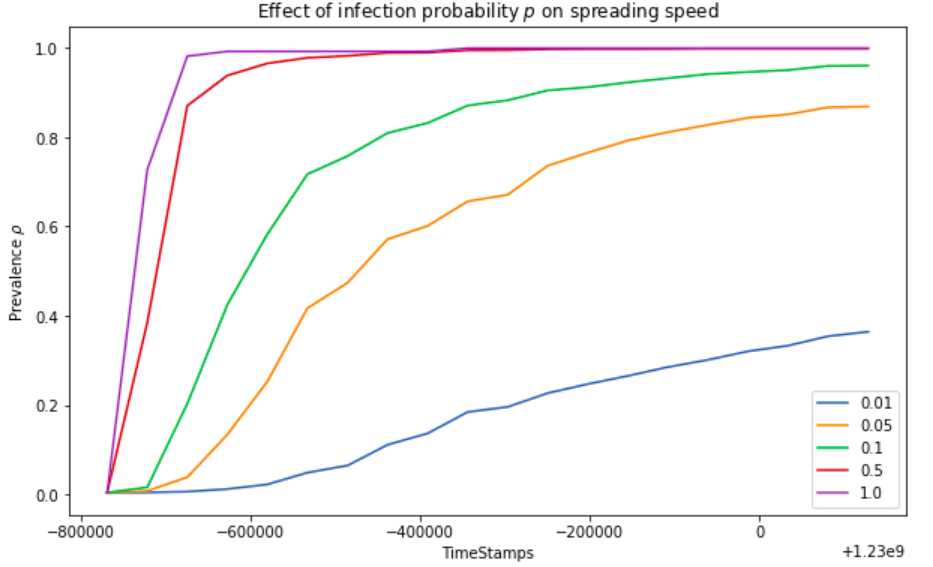
\includegraphics[width=0.5\textwidth]{q2}
\end{center}

\textbf{b)}  For which infection probabilities does the whole network become fully infected?
What are the stepwise, nearly periodic “steps” in the curves due to?

\bigskip
\textbf{Ans: }The probabilies $p=0.5$ and $p=1$ results in the whole network being infected.
The period steps might be due a hub being infected hence, causing a higher dispersal of the infection (hubs have
more neighbours)

\section{Effect of seed node selection on spreading speed}
Next, we will investigate how the selection of the seed node affects the spreading speed.

\bigskip
\textbf{a)} Use nodes with node-ids [0, 4, 41, 100, 200] (ABE, ATL, ACN, HSV, DBQ) as
seeds and p = 0.1, and run the simulation 10 times for each seed node. Then, plot the
average prevalence of the disease separately for each seed node as a function of time.

\begin{center}
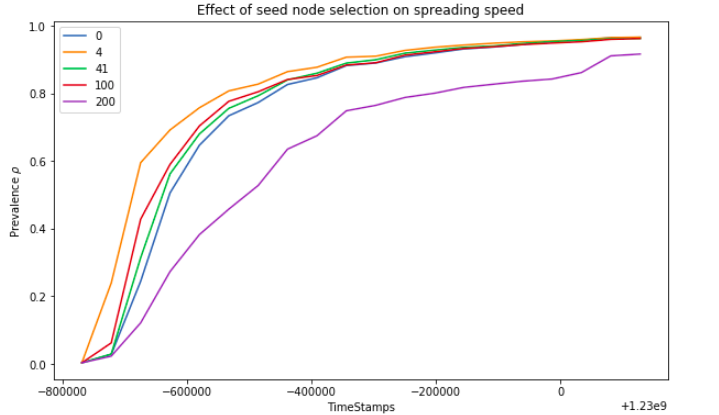
\includegraphics[width=0.5\textwidth]{q3}
\end{center}

\textbf{b)} You should be able to see differences in these spreading speed. Are these differences visible in the beginning of the epidemic or only later on? Why?

\bigskip
\textbf{Ans: }The differences are more visible at the beginning of the epidemic. Later on, most of the prevalence converge to around 96% (except for choosing node 200)

After overcoming advantages of choosing certain more well connected nodes, the spread speed reached an equilibrium.

\bigskip
\textbf{c)} In the next tasks, we will, amongst other things, inspect the vulnerability of a node for becoming infected with respect to various network centrality measures. Why is it important to average the results over different seed nodes?

\bigskip
\textbf{Ans: }Different seed nodes can affect the spread seed and the vulnerability of a node is not easily observable at first. For example, some nodes are isolated (such as node )
hence, takes some
time before the infection reaches a hub and spreads quickly. This transient time accounts for
much of the variance.

\section{Where to hide?}
Now, consider you want to be as safe from the epidemic as possible. How should you select
your refuge? To answer this question, run your SI-model 50 times with p = 0.5 using different
random nodes as seeds and record the median infection times of each node. Note that the
median infection time is not well defined for nodes that become infected in less than 25 runs.
You may leave those nodes out from your analyses.

\bigskip
\textbf{a)} Run the 50 simulations, and create scatter plots showing the median infection time
of each node as a function of the following nodal network measures:

i) k-shell

ii) unweighted clustering coefficient c

iii) degree k

iv) strength s

v) unweighted betweenness centrality

vi) closeness centrality

  \begin{minipage}{0.5\textwidth}
    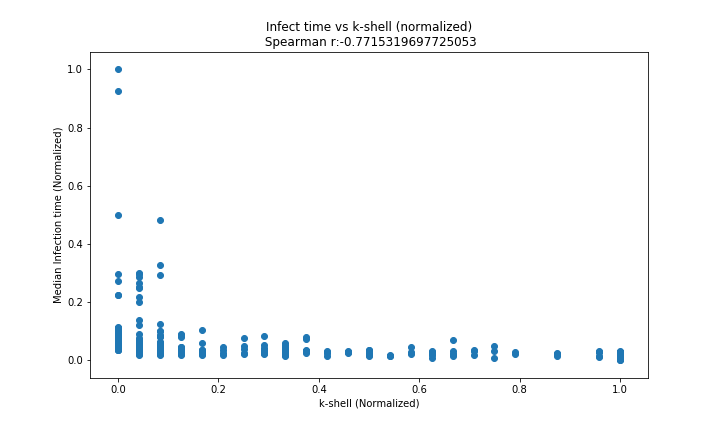
\includegraphics[width=\textwidth]{0}
  \end{minipage}
  \begin{minipage}{0.5\textwidth}
    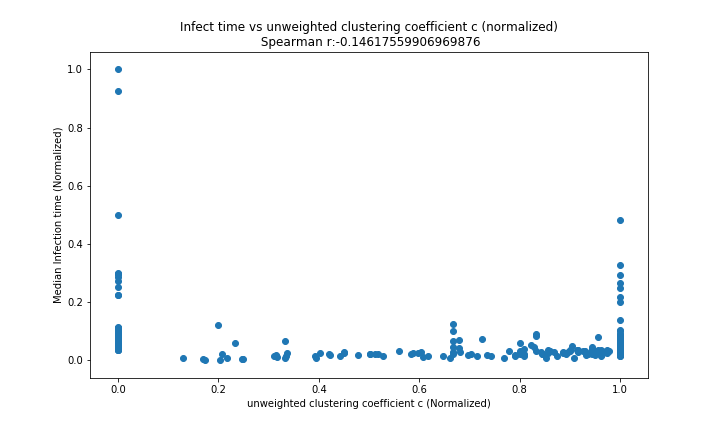
\includegraphics[width=\textwidth]{1}
  \end{minipage}
  \begin{minipage}{0.5\textwidth}
    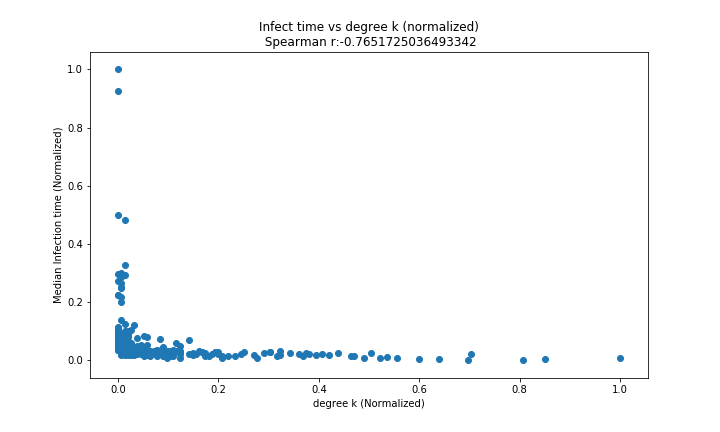
\includegraphics[width=\textwidth]{2}
  \end{minipage}
  \begin{minipage}{0.5\textwidth}
    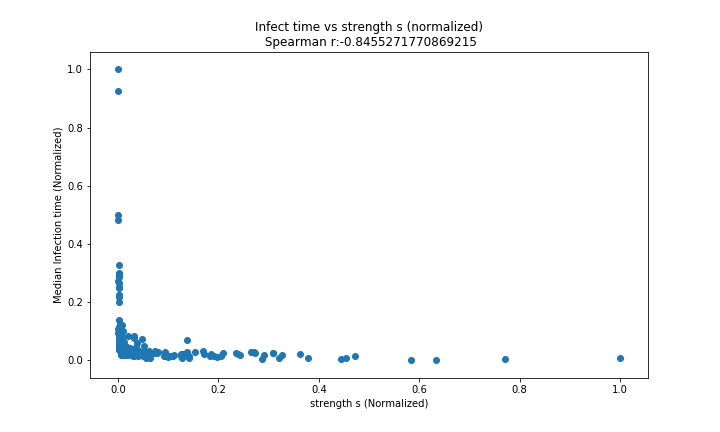
\includegraphics[width=\textwidth]{3}
  \end{minipage}
  \begin{minipage}{0.5\textwidth}
    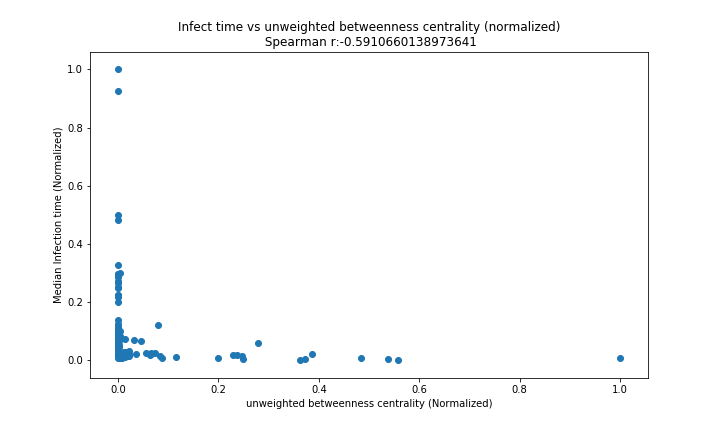
\includegraphics[width=\textwidth]{4}
  \end{minipage}
  \begin{minipage}{0.5\textwidth}
    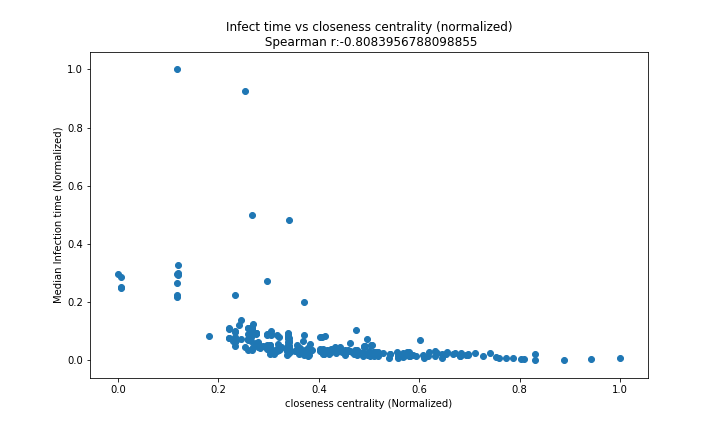
\includegraphics[width=\textwidth]{5}
  \end{minipage}

\clearpage
  
\textbf{b)}  Use the Spearman rank-correlation coefficient  for finding out, which of the
measures is the best predictor for the infection times

\bigskip
\textbf{Ans: }
\begin{table}[h]
  \begin{tabular}{|c|c|}
    \hline
    Measure & Spearman rank-correlation coefficient $\rho$ \\ \hline \hline
    k-shell & -0.772 \\ \hline
    unweighted clustering coefficient c & -0.146 \\ \hline
    degree k & -0.765 \\ \hline
    strength s & -0.846 \\ \hline 
    unweighted betweenness centrality & -0.591 \\ \hline
    closeness centrality & -0.808 \\ \hline
 \end{tabular}
\end{table}

\textbf{strenght s} ($\rho$: -0.845) and \textbf{closeness centrality} ($\rho$: -0.808)
seems better predictors for infection times

\bigskip
\textbf{c)} Discuss your results for each network centrality metric.
Especially, explain the ranking of the network measures as measured by the median infection
time.

\textbf{Ans:} \textbf{closeness centrality} ($\rho$: -0.808) is a measure of how centrality
a node is and how close it is to other nodes. Thus, it will get infected faster relative
to nodes who are less central since it is easier for the disease to get to this node.

\bigskip
\textbf{strenght s} ($\rho$: -0.845) this is also a good indicator. Strength is a sum
of weights of edges adjacent to the edge. Edge with high strength 1) Hubs
that are connected to many nodes in the region and 2) entry points to the region
from a node that is relatively far away. Thus, these nodes are easier to infect quickly.
\textbf{Degree} is very similar except it is not weighted. Thus, we have less information and
is not as good as strength as a measure.

\bigskip
\textbf{Unweighed cluster coefficient} is the worst as it provides not as much information
of the node and its neighbours.

\section{Shutting down airports}
Immunization strategy:

- random neighbour (bump up the prob of hubs)

- random immunizaion

- highest 'k-shell'

- highest 'unweighted clustering coefficient c'

- highest 'degree k'

- highest 'strength s'

- highest 'unweighted betweenness centrality'

- highest 'closeness centrality'

\bigskip
\textbf{a)} adapt your code to enable immunization of nodes, and plot the prevalence of the
disease as a function of time for the 8 different immunization strategies (social net., random
node, and 6 nodal network measures) when 10 nodes are always immunized.

\begin{center}
  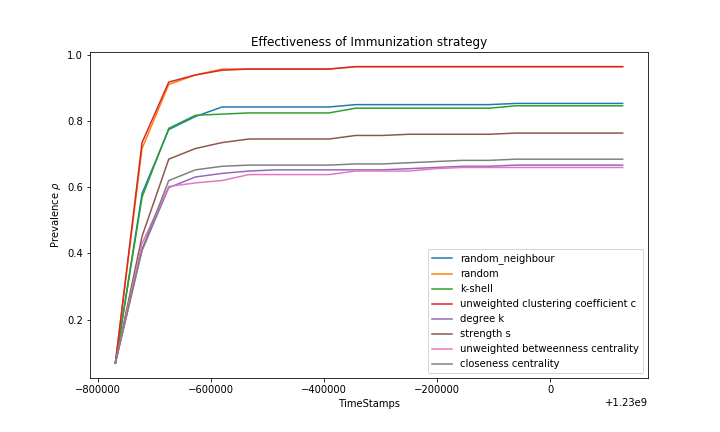
\includegraphics[width=0.8\textwidth]{immune_strategy}
\end{center}

\textbf{b)} Discuss the ranking of the immunization strategies. In particular, compare your
immunization results with the results you obtained in the previous task (Task 4). Are
there some measures that are bad at predicting the infection time but important with
regards to immunization? Or vice versa? Why?

\textbf{Ans: }
\begin{table}[h]
  \begin{tabular}{|c|c|c|}
    \hline
    Measure & Spearman  $\rho$ & Infection Ratio\\ \hline \hline
    k-shell & -0.772 & 0.846\\ \hline
    unweighted clustering coefficient c & -0.146 & 0.964\\ \hline
    degree k & -0.765 & 0.667\\ \hline
    strength s & -0.846 & 0.763\\ \hline
    unweighted betweenness centrality & -0.591 & 0.659\\ \hline
    closeness centrality & -0.808 & 0.685 \\ \hline
 \end{tabular}
\end{table}
\begin{center}
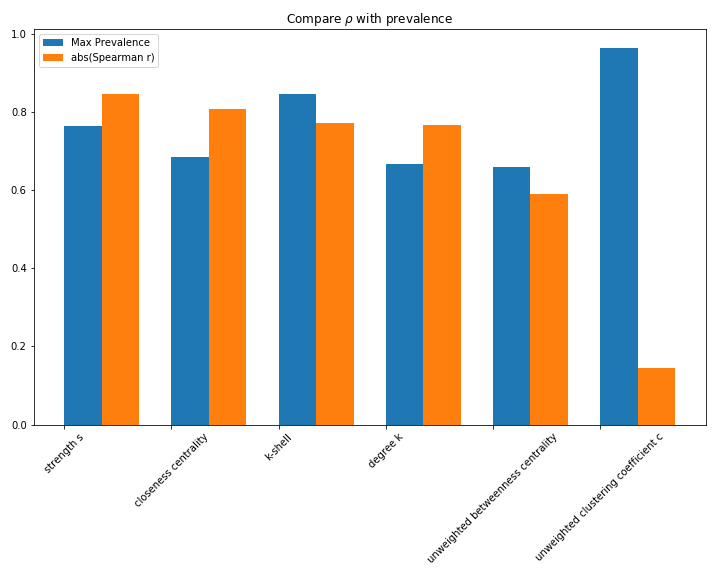
\includegraphics[width=0.5\textwidth]{compare}
\end{center}


Closeness centrality is the best measure in predicting infection. By targetting
the nodes with the highest closeness centrality, we can hinder the infection because since
it is a measure of how close it is to other nodes.  These nodes tend to be airports
that happens to be in most shortest path.

On the other hand, cluster coefficient is not a good measure and targetting nodes
with higher coefficient does not inhibit the spread.

\bigskip
\textbf{c)}  The network immunization strategy suggested for use in social networks should
have worked better than the random node immunization . Let us next explain this mathematically
by investigating the probability of picking high-degree nodes at random and by
the social net immunization strategy:

\bigskip
Probability of picking a random node with degree k $= \frac{1}{N}$ where $N$ is the number
of nodes in the graph

\bigskip
Probability to pick a node with degree k by the social net immunization strategy
$\frac{1}{N} \times \frac{degree}{\text{total edges}}$

Thus, social network immunization has higher probability since you increase
the chances of choosing a node
with a high degree (maybe a hub)


\bigskip
d) (1 pt) Although the social network immunization strategy outperforms the random
immunization, it is not as effective as some other immunization strategies.
Explain, why it still makes sense to use this strategy in the context of social networks?

\textbf{Ans: }It is the easiest to implement as it does not require much information about
the node. You can apply it to any node indiscriminately.


\clearpage
\section{Disease transmitting links}

\textbf{a)} Run the simulations, and compute the fraction of times each link is used for infecting
the disease ($f_{ij}$ ). Then visualize the network on top of the US map. Adjust the width of
the links according to the fractions $f_{ij}$ to better see the overall structure:

\begin{center}
  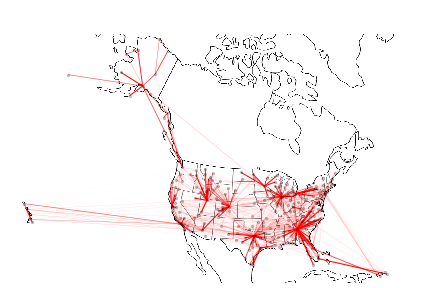
\includegraphics[width=0.8\textwidth]{usa}
\end{center}

Compare your
visualization with the \textbf{maximal spanning tree} of the network below.

\begin{center}
  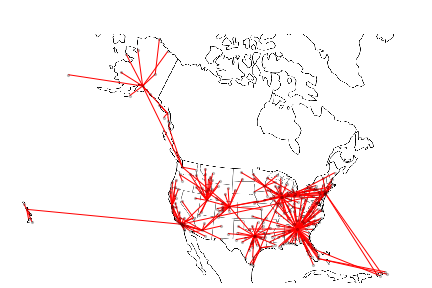
\includegraphics[width=0.8\textwidth]{plot_mst.png}
\end{center}

\textbf{b)} What do you notice? How would you explain your finding?

\bigskip
\textbf{Ans: }The mst and our graph happens to coincide with each other approximately. Since maximal spanning tree has all edges and the max weight, to obtain this max weight, we reach a hub can traverse the edges to nodes in the region.

This is similar to how disease spreads quickly, by infecting a hub and infecting the region.

\bigskip
\textbf{c) }Create scatter plots showing $f_{ij}$ as a function of the following link properties:

i) link weight $w_{ij}$

ii) link neighborhood overlap $O_{ij}$

iii) \textit{unweighted} link betweenness centrality $eb_{ij}$

  \begin{minipage}{0.5\textwidth}
    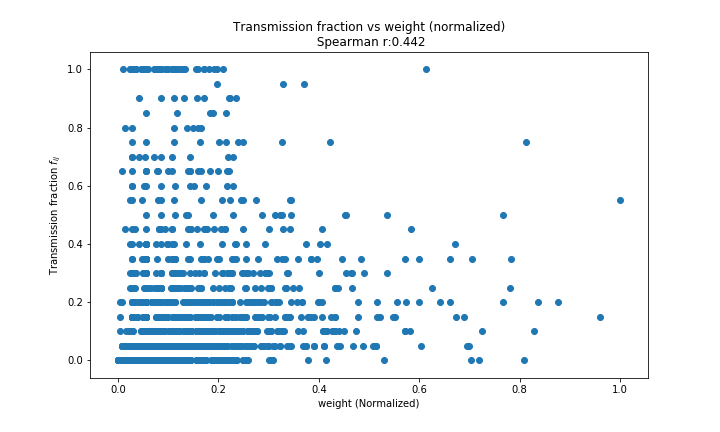
\includegraphics[width=\textwidth]{weight}
  \end{minipage}
  \begin{minipage}{0.5\textwidth}
    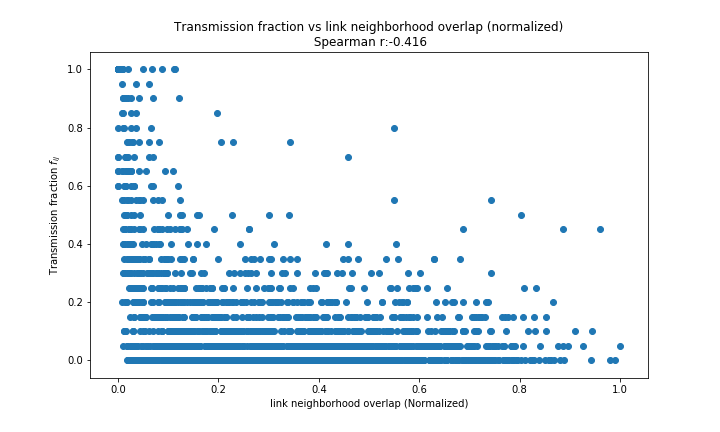
\includegraphics[width=\textwidth]{overlap}
  \end{minipage}
  \begin{minipage}{0.5\textwidth}
    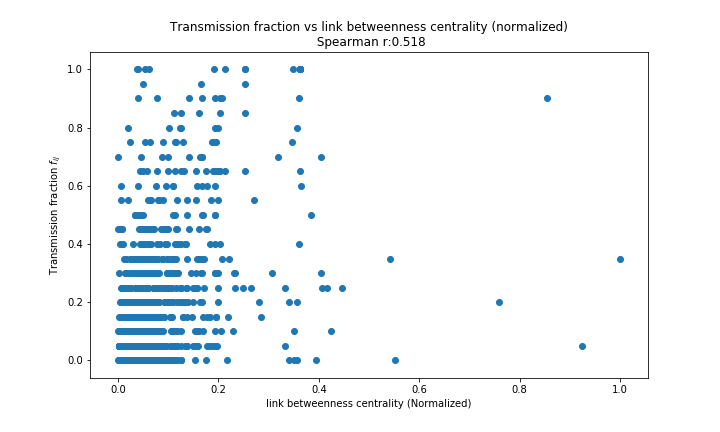
\includegraphics[width=\textwidth]{linkbetweenness} 
  \end{minipage}

Compute also the Spearman correlation coefficients between f ij and the three link-wise
measures.

\begin{table}[h]
  \begin{tabular}{|c|c|}
    \hline
    Link Measure & Spearman  $\rho$ \\ \hline \hline
    Weight & 0.441 \\ \hline
    link neighborhood overlap & -0.416 \\ \hline
   link betweenness centrality &0.518  \\ \hline
 \end{tabular}
\end{table}

\textbf{d)}  Explain the performance of the three link properties for predicting $f_{ij}$ .

\textbf{Ans: }All 3 measures are not too food in predicting $f_{ij}$. Link betweenness
it the best performing because
it is the sum of the fraction of all-pairs shortest paths that pass through the link.

\section{BONUS task}

None of the above measures was extremely good for predicting $f_{ij}$ . As a bonus task, you can
come up with a measure of your own, or find out an appropriate measure from the literature that
you think is better for predicting $f_{ij}$ than the three measures listed above. Motivate selection of method, and perform similar investigations as with the other link properties. Especially evaluate the Spearman correlation between the measure you developed and $f_{ij}$ . fraction of times each link is used for infecting the disease ($f_{ij}$).

\bigskip
\textbf{Suggestions: } We can take a look at whether the edge is also an element of
the maximal spanning tree. and also make use of the link betweenness centrality of
the links

  \begin{minipage}{0.5\textwidth}
    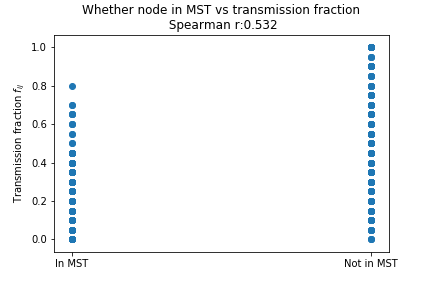
\includegraphics[width=\textwidth]{mst}
  \end{minipage}
  \begin{minipage}{0.5\textwidth}
    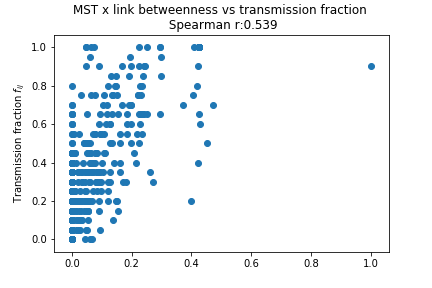
\includegraphics[width=\textwidth]{mstbetween}
  \end{minipage}

  Both increase transmission fraction $f_{ij}$ insignificantly.

  The spearman correlation in 
  the MST method increase to 0.532 while the MST x link betweenness centrality increase
  to 0.539, albeit insignificantly..

  \section{Graph Clustering}

  Clustering similar nodes together.

  \textbf{input}: graph adjacency matrix $A$, number $k$
  
  1. form diagonal matrix $D$
  
  2. form unnormalized Laplacian $L = D − A$
  

  3. compute the first $k$ eigenvectors $u_1 , \dots, u_k$ of the \textit{generalized eigenproblem} $L \mathbf{u} = \lambda D \mathbf{u}$ (eigenvectors of $L_{rw}$)

  4. form matrix $U \in \texttt{R}^{n \times k}$ with columns $u_1, \dots, u_k$
  
  5. Normalize $U$ such that rows have norm 1
  
  6. consider the i-th row of $U$ as point $y_i \in \texttt{R}^k, \; i=1, \dots, n$
  
  7. cluster (kmeans) the points $\{y_i\}_{i=1, \dots, n}$ into clusters $C_1, \dots, C_k$
 
  \textbf{output} clusters $A_1, \dots A_k$

  Here, $L_{rw} := I - D^{-1} A$

  \begin{center}
  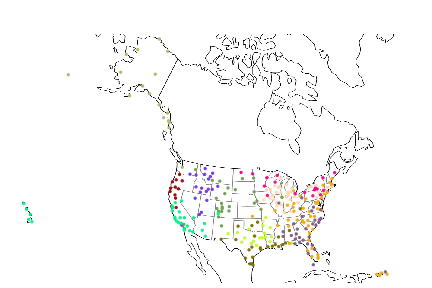
\includegraphics[width=0.8\textwidth]{cluster}
\end{center}

Nodes with similar locations in the graph can be clustered together.
\end{document}